\chapter{Overview}
\label{chap:overview}

In this section, I provide an overview of some of the essential concepts used in this project, illustrated through the following thought experiment:

Carol, Dave, and Trent are playing a game. In each iteration of the game, Trent will present Carol with some raw data in some format (for example, results of coin flips, or randomly chosen letters) and Carol will try to communicate the data to Dave (who is in the next room) as briefly as possible. Carol and Dave are communicating through a channel that allows only 0s and 1s to be sent. Carol and Dave each know the format of the data and are allowed to coordinate on a strategy for communication before the game starts. In fact, Carol and Dave are so good at this coordination that we may assume that everything Carol knows before the game starts, Dave also knows.

For an example, let us say that the data Trent is presenting to Carol is the result of a sequence of fair coin flips in the format "heads, tails, tails, ..." Because they each know the format, a simple strategy would be to use a \textbf{code} where heads are denoted by 0s and tails are denoted by 1s over their communication channel. We refer to the result of each coin flip as a \textbf{symbol}, and in this example we see that the \textbf{code rate} is 1 bit per symbol.

In this example, symbols are \textbf{independent and identically-distributed random variables (i.i.d.)} because each coin flip has the same 50-50 chance of coming up as heads or tails (identical distribution) and because the result of one coin flip doesn't affect any other (independence).

\section{Information and entropy}
\label{sec:information_and_entropy}

Before attempting to compress a work of literature, let us first think about individual letters.

In another instance of the previous game, Trent presents Carol with a sequence of letters, each randomly chosen from a large English text. As before, symbols are independent and identically-distributed, but in this case, the distribution is not uniform, since the letter E occurs much more often than the letter Q.

As well as saying that Q has a low probability, it is sometimes said that Q has high \textbf{surprisal}. Because of this, Carol and Dave would be wise to privilege the letter E with a short representation in their code (say \texttt{00}), because it will occur often, and vice versa. Because this will leave Q with a longer code, we also say that Q has high \textbf{(self-)information}.

In his seminal paper "A Mathematical Theory of Communication", \textcite{shannon1948mathematical} defines the \textbf{information content} of a symbol as length of its binary representation when the symbol code is chosen optimally (estimated as $-\log p(x)$, where $p(x)$ is the probability of that symbol), and defines the \textbf{entropy} of a random variable (such as our symbols) as the average amount of information per symbol, given by

\[H(X) = \mathbb{E}[-\log p(X)] = -\sum_{x \in \mathcal{X}} p(x) \log p(x)\]

for the discrete random variable $X$. In simple terms, the entropy of a variable is the average number of yes/no questions one needs to ask to determine the value of that variable when choosing one's questions optimally. For a fair coin, one needs to ask only one yes/no question to learn the outcome, and so the entropy of that outcome is 1 bit (sometimes called 1 shannon).

For the English language, the entropy of individual letters based on their frequency is known to be approximately 4.14 bits. This value indicates that, if one person were to select a letter at random from an English text and another person were to try to guess it by asking only yes/no questions optimally, they would need to ask 4.14 questions on average.

The importance of this value is related to Shannon's \textbf{source coding theorem}, given in the same paper, which shows that no code can be chosen for which the code rate is less than the entropy of the symbols in question.

In our example with randomly-chosen English letters, the calculated entropy of English letters indicates that no code that Carol and Dave can choose can have a lower code rate than 4.14 bits per symbol. But how might they go about constructing a minimal code?

\section{Entropy coding}

An \textbf{entropy coding} is a consistent way of assigning binary sequences to symbols. Entropy codes usually aim at being minimal in the sense that an encoding of a stream of symbols that the code is designed for should have an average code rate that approximates the symbols' entropy.

The codes are generated from an input mapping between the potential values of each symbol and that value's probability. For example, a coding algorithm may take as its input the mapping $\{A \rightarrow 0.8, B \rightarrow 0.15, C \rightarrow 0.05\}$ and output the mapping $\{A \rightarrow \texttt{0}, B \rightarrow \texttt{10}, C \rightarrow \texttt{11}\}$. Two of the most commonly used entropy codings are Huffman coding and arithmetic coding.

\subsection{Huffman Coding}

\begin{wrapfigure}{r}{0.3\textwidth}
    \centering
    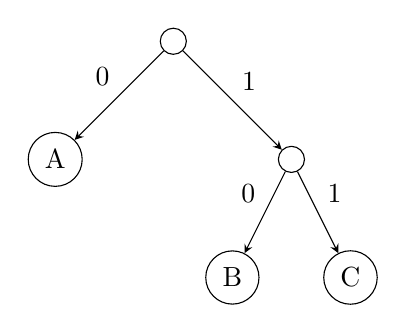
\begin{tikzpicture}
        [->,>=stealth,level/.style={sibling distance = 3cm/#1, level distance = 1.5cm}]
        \node [circle,draw] (root) {} % root node, unlabeled
        child { node [circle,draw] (A) {A} 
            edge from parent node[above left] {0} % Label on the arrow to A
        }
        child { node [circle,draw] (mid) {} % Unlabeled node
            child { node [circle,draw] (B) {B} 
                edge from parent node[above left] {0} % Label on the arrow to B
            }
            child { node [circle,draw] (C) {C} 
                edge from parent node[above right] {1} % Label on the arrow to C
            }
            edge from parent node[above right] {1}
        };
    \end{tikzpicture}
\end{wrapfigure}

Huffman coding works by recursively combining low-probability symbols into a set of symbols that share the same prefix. For example, when given the input $\{A \rightarrow 0.8, B \rightarrow 0.15, C \rightarrow 0.05\}$, Huffman coding combines the symbols B and C into a group that will share the prefix \texttt{1} and which, as a whole, has probability 0.2 .

For this project, I use my own implementation of Huffman coding in the \texttt{Huffman} class available for viewing at \texttt{\href{https://github.com/Guy29/FYP/blob/main/Code/libraries/codes.py}{libraries/codes.py}}. More detail on this implementation is available in section \ref{subsec:n_gram_practical}.

\subsection{Arithmetic Coding}

Arithmetic coding is a method where the cumulative probability of symbols is calculated (i.e. $\{\emptyset \rightarrow 0, \{A\} \rightarrow 0.8, \{A,B\} \rightarrow 0.95, \{A,B,C\} \rightarrow 1\}$) and a range within the interval $[0,1)$ is given in a binary format to indicate one of the symbols.

My implementation of arithmetic coding is also available at \texttt{\href{https://github.com/Guy29/FYP/blob/main/Code/libraries/codes.py}{libraries/codes.py}}.

\section{Regularity and the importance of context}
\label{sec:regularity_and_context}

Let's now imagine yet another instance of the game. In this version, the data Trent gives to Carol is a sequence of English letters making up a novel. In this case, our symbols are again letters, and the previously used code designed for randomly chosen English letters can be used with some success. However, that code is no longer optimal.

This is because the symbols given by Trent are no longer independent or identically distributed, that is, letters cross-correlate. For example, whenever the letter Q appears in the sequence of symbols, there is a high probability that the following symbol will be U, by the structure of English. This \textbf{regularity} can be exploited in Carol and Dave's choice of code, so that whenever the symbol Q is encountered, the symbol U is given a shorter code within that \textbf{context} to reflect its high probability.

In the extreme case where each Q is necessarily followed by a U, Carol and Dave's code may not assign U a code at all, as it can be immediately inferred whenever a Q is encountered. In this case, it can be said that the regularity of QU has been \emph{abstracted out} in the encoded version of the text. The result of this abstraction is a version of the text with less regularity and with higher entropy, that is, a more information-dense representation.

In fact, we should expect a perfect coding - one that removes all regularity from the text to be transmitted - to result in a sequence of bits which contain no regularity whatsoever and which is maximally entropic (i.e. every sequence is as likely as every other), and which is therefore indistinguishable from noise.

For example, an ideal coding may abstract out the tense in the sentence "Yesterday I ate a sandwich" by noting the correlation between "yesterday" and "ate", and may represent this tense once in the coding instead of have it repeated, for example by transmitting \texttt{"(day) I (eat) a sandwich" + (day = yesterday)}. Because the redundancy has been removed and the day is only indicated in one place, it now becomes possible to alter the value of the day to "tomorrow" and obtain the decoding "Tomorrow I will eat a sandwich" instead of landing in the inconsistent state "Tomorrow I ate a sandwich".

Because of this, we should expect that - if Carol and Dave use a coding which exploits regularities in the text - then sending Dave a random sequence of bits should result in a decoding that is still consistent to those regularities. This is shown empirically in Figures \ref{fig:predictor_decoding_randomness} and \ref{fig:ML_decoding_randomness}.


In essence, such a coding would be implementing the advice sometimes given to programmers of "making illegal states unrepresentable", and by extension yielding the contrapositive of making every representable state legal.

\section{Prediction and compression}

So far we have discussed this thought experiment in terms of Carol and Dave agreeing on a strategy for communication before the game starts, conceptualized as a set of specific codes that apply within corresponding contexts. This is not in fact necessary, and \textcite{Shannon1951} proposes an alternative mode illustrated in Figure \ref{fig:twin_communication}.

\begin{figure}[h]
\centering
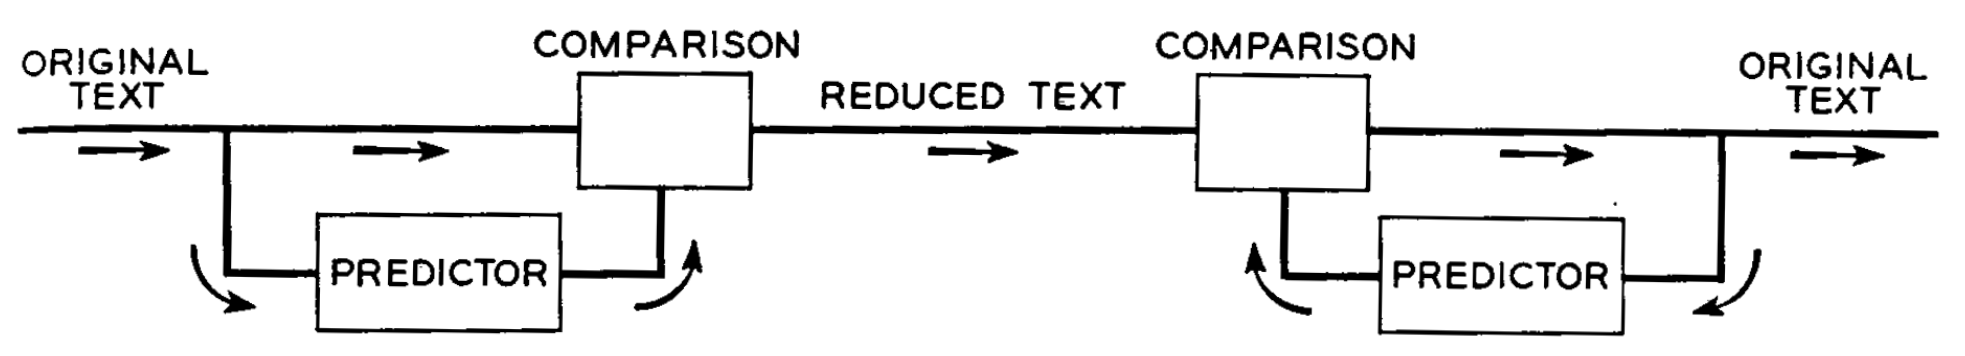
\includegraphics[width=\textwidth]{img/twin_communication.png}
\caption{Shannon's illustration, titled "communication system using reduced text"}
\label{fig:twin_communication}
\end{figure}

In this mode, we imagine Carol and Dave starting off with identical mental states, something which is unlikely in practice but easily implementable in silico. Instead of pre-agreeing to a code, the encoding happens in the following way:
\begin{itemize}
    \item Carol reads the text, constantly making predictions about what the next symbol will be before reading it by ranking all the possibilities. She simply writes down the rank of the character which turned out to be correct. For example, if she reads the word "queue" she may note it down as the sequence "15, 1, 2, 1, 1", indicating that the Q was 15th in order of expectation, the following U was 1st, etc. These numbers are then transmitted to Dave.
    \item Dave performs a symmetrical process of listing his expectations for the next letter (these expectations should be identical to Carol's at every point, since they start off from identical mental states and update their mental states on the same stream of characters), reading the rank sent over by Carol, and writing down the letter that corresponds to that rank in his own ranking of symbols.
\end{itemize}

Shannon's original formulation used numbered ranks in transmission because it facilitates analysis, but practical systems inspired by this method may instead use an entropy code, and later I implement a \texttt{Compressor} class, initialized with \texttt{Predictor} and a \texttt{Code} objects that implement this scheme. \texttt{Predictor} objects in this code also generate probability ranks for a text on request, as illustrated in Figure \ref{fig:predictor_surprisal_by_char}.

\section{Last thoughts}

Note the similarity between this encoding method and the concept of AIXI presented in section \ref{sec:motivation}. In each of these, predictions about next observations are made based on a prior, a real observation is made, and internal models are updated in a way that minimizes future surprisal. In Carol and Dave's case, having a good understanding of the text and being able to make good predictions about future observed symbols is desirable because in effect they only need to encode deviations between reality and expectation, and therefore have an interest in minimizing that deviation, while in AIXI's case good predictions are adaptive as they help maximize rewards.

In the field of neural network-based machine learning, prediction and correction correspond to forward propagation and backpropagation, and a simple application of neural networks for compression is given in section \ref{sec:machine_learning}.

Further to the biological side, a current hypothesis in the field of neuroscience relates to this idea, namely \textbf{predictive coding}, also known as predictive processing. \textcite{millidge2021predictive} define predictive coding as the postulate that \textquote{the core function of the brain is simply to minimize prediction error, where the prediction errors signal mismatches between predicted input and the input actually received} and mention that minimization is achieved through \textquote{immediate inference about the hidden states of the world} and \textquote{updating a global world-model to make better prediction}. Similarly, \textcite{clark2013whatever} gives the function of brains as \textquote{constantly attempting to match incoming sensory inputs with top-down expectations or predictions. This is achieved using a hierarchical generative model that aims to minimize prediction error.} The aforementioned Anil Seth and Andy Clark are major figures in the field of predictive coding.

One of the seminal works in the field of cognitive neuroscience which contains an early concept of predictive coding is that by \textcite{mcclelland1981interactive}, titled "An Interactive Activation Model of Context Effects in Letter Perception". In this paper, the authors write \textquote{we assume that perception is fundamentally an interactive process. That is, we assume that "top-down" or "conceptually driven" processing works simultaneously and in conjunction with "bottom-up" or "data driven" processing to provide a sort of multiplicity of constraints that jointly determine what we perceive.}

Lastly, note that AIXI differs from a simple encoder in that it also takes action in its world, affecting its state. It therefore has one more method by which to minimize surprise, as it can nudge its world in a direction it is better able to predict. As with predictive coding, there is a supporting hypothesis from neuroscience, namely active inference, which extends predictive coding. While predictive coding deals with how the brain processes incoming data (perceptions), active inference addresses the outgoing signals of the brain (actions), and within its model actions are also attempts at bringing the observed world in line with predicted world by changing the former instead of the latter.
